\chapter{Software-Entwicklung und Experimente}
Aus den anfänglichen Ideen für die Umsetzung des Lighthouse Keeper entstehen in diesem Kapitel die ersten Module für dessen Verwirklichung. Zum Anfang wird die verwendete Hardware vorgestellt und in Verbindung dazu die genutzten Software-Komponenten. Durch die geeignete Wahl aller Bestandteile, lassen sich viele Aufgaben auf vorgefertigten Module übertragen. Beispielsweise werden statt einer eigenen Entwicklung, ein bestehendes Kommunikations-Framework und eine bereits existierende Middleware für den Roboter genutzt. Mit der Nutzung dieser fertigen Lösungen wird im großen Maße Arbeitsaufwand eingespart und ermöglicht einen stärkeren Fokus auf das eigentliche Thema. Da dies im Hinblick auf die Smartphone-Applikation nicht immer möglich war, wird deren Implementierung in diesem Kapitel exemplarisch einmal dargestellt. \\ \\
Die durchgeführten Experimente beziehen sich in diesem Teil der Arbeit auf die Messung der Signalstärke der Beacons in Abhängigkeit zu deren Entfernung. Diese Phase in der Prozessplanung legt den Grundstein für die Modellbildung, welche anschließend im nächten Kapitel vorgenommen wird. Ferner werden einzelne Einflüsse auf die Messungen näher betrachtet und eine Analyse zu der Batterielaufzeit eines Beacons in Abhängigkeit zu seinen Einstellungen aufgestellt.
\section{Verwendete Hardware}
Da die Beacon-Technologie vorrangig zur Indoor-Lokalisierung von Personen eingesetzt wird und als Peripheriegerät meistens ein Smartphone Verwendung findet, wird auch ein solches für die gesamte Testdauer als Messgerät genutzt. Die Wahl fiel dabei auf ein Android-Smartphone mit dem Namen Motorola Moto G der gleichnamigen Firma Motorola Inc. Es wurde ausgewählt, weil es alle Hardware- und Software-Anforderungen zum Empfang von BLE-Signalen erfüllt und als ein Standard-Smartphone gilt, sodass sich mit den ihm erzielten Ergebnisse auch auf andere Produkte übertragen lässt. Desweiteren werden zwei Roboter in den Experimenten genutzt, um die Messungen reproduzierbar und standardisiert durchzuführen. Für die reinen Distanz-Signalstärke-Messungen wird der Roboters bzw. lediglich sein Arm namens "`Youbot"' der Kuka AG und später für die Validierung einer Beacon-Konfiguration der Roboter "`Scitos G5"' der MetraLabs GmbH verwendet. 
\subsection{Motorola Moto G}
Das Moto G dient als Empfangsstation der BLE-Signale, dessen grundlegende Spezifikationen ein 1,2 GHz Snapdragon 400 Prozessor mit 1 GB RAM und ein WCN3620 BT/FM/WLAN RF Modul aussmachen (\cite{Moto}). Desweiteren verwendet es standardmäßig ein Android 4.3 als Betriebssystem, welches jedoch für die Experimente auf die Version 4.4 geupdated wurde. Neben der technischen Austattung und Software sind für die späteren Messungen die Antennen und deren Charakteristiken von hoher Bedeutung, denn deren Eigenschaften wirken sich direkt auf den Empfang der Signale aus. Um die Einflüsse besser zu verstehen, sind in den Abbildungen \ref{fig:MotoGV} und \ref{fig:MotoA} die Anordnung der Antennen einmal skizziert. Dabei fällt es auf, dass sich WLAN- und Bluetooth-Modul die selben Antennen teilen. Dies führt zu der Frage, ob es zu Konflikten in der Funktionsweise des Smartphones kommt, wenn gleichzeitig auf beide Module zugegriffen wird. Jedoch dazu mehr im Abschnitt der App-Entwicklung. Die zweite Frage die sich daraus stellt, ist die Veränderung der Empfangs- und Sendequalität des Moto G in verschiedenen Positionen. Eine Antenne hat je nach Bauform und Funktionsweise Bereiche, in der sie mit voller leistung sendet und empfängt, aber auch Bereiche in der Funk-Signale sie weder verlassen noch erreichen können. Das hat verschiedene physikalische Gründe, jedoch sind diesen komplexen nichtlinearen Eigenschaften der Antennen des Moto G zumindest nicht öffentlich bekannt und können auch nicht einfach bestimmt werden. Es sei nur anzumerken, dass bei den Messungen auch darauf geachtet werden muss, wie und an welchen Halte-Punkten das Moto G am besten befestigt wird, ohne deren Transceiver-Fähigkeiten negativ zu beeinflussen. Eine gute Annahme dabei ist es das Smartphone so auszurichten, als ob es flach in der Hand eines Menschen liegen würde. Der Hersteller wird schließlich darauf bedacht sein, sein Produkt für einen normalen Betrieb auszulegen und somit auch die Konstruktion und Bau der Antennen danach optimieren. Diese Annahme muss jedoch noch anhand von Messungen verifiziert werden.
\begin{figure}[t!]
$\begin{minipage}[b]{7cm}
\centering
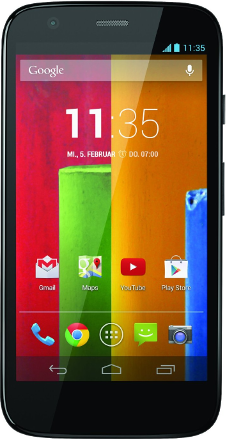
\includegraphics[width=0.45\textwidth]{Bilder/MotoG} 
\caption{Vorderseite des Motorola Moto G \cite{MotoGV}}
\label{fig:MotoGV}
\end{minipage}
\hfill
\begin{minipage}[b]{7cm}
\centering
\begin{tikzpicture}
\node [anchor=south west,inner sep=0] at (0,0) {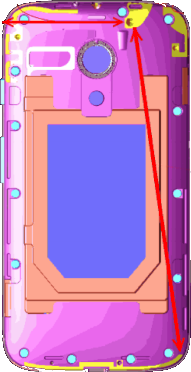
\includegraphics[width=0.45\textwidth]{Bilder/MotorolaAntenne}};
\draw [red,-angle 60,line width=0.49mm] (2.4,5.77) -- (3.375,5.77);
\node (1) at (3.375,5.77) {};
\node [right=0.1cm of 1,inner sep=0, text width = 4cm] {Bluetooth- und WLAN-Antennen};
\end{tikzpicture}
\caption{Rückseite vom Moto G mit Antennen-Gerüst  \cite{Moto}}
\label{fig:MotoA}
\end{minipage}$
\end{figure}
\subsection{Youbot}
In vorigen Abschnitt wurde schon angesprochen, dass die Lageposition des Messinstrumentes zu seiner Empfangsleistung überprüft werden muss. Zudem soll das Smartphone so gehalten werden, als wenn es sich in einer flachen Hand befindet und so auch die Experimente durchgeführt werden. Um all dies zu erreichen und auch unter der Anforderung an einen automatisierten und reproduzierbaren Prozess, empfiehlt es sich einen Roboterarm als Mess-Plattform zu benutzen. Aufgrund der Verfügbarkeit wurde das Modell "`Youbot"' der Firma "`Kuka"' gewählt und für die Messungen mit einer Halterung aus einem 3D-Drucker regänzt (siehe Abbildung \ref{fig:Youbot1}). Die Vorteile des Systems sind zum einen der hochpräzise Roboterarm auf dem Youbot und zum anderen, dass ein vollwertiger Rechner mit einem Linux Betriebssytem im System verbaut ist und so die Kommunikation zwischen zentralem Computer sehr einfach aufgebaut werden kann. Der künstliche Arm kann sich um fünf Achsen drehen (siehe Abbildung \ref{fig:Youbot2}) und bietet somit genug Möglichkeiten, die Lageposition vom Moto G zu verändern. 
\begin{figure}[H] 
$\begin{minipage}[b]{7cm}
\centering
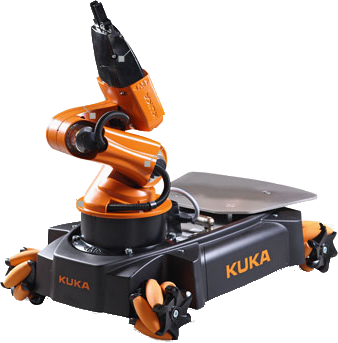
\includegraphics[scale=0.07]{Bilder/Youbot}
\caption{Youbot mit Halterung (gelber Aufsatz)}
\label{fig:Youbot1}
\end{minipage}
\hfill
\begin{minipage}[b]{7cm}
\centering
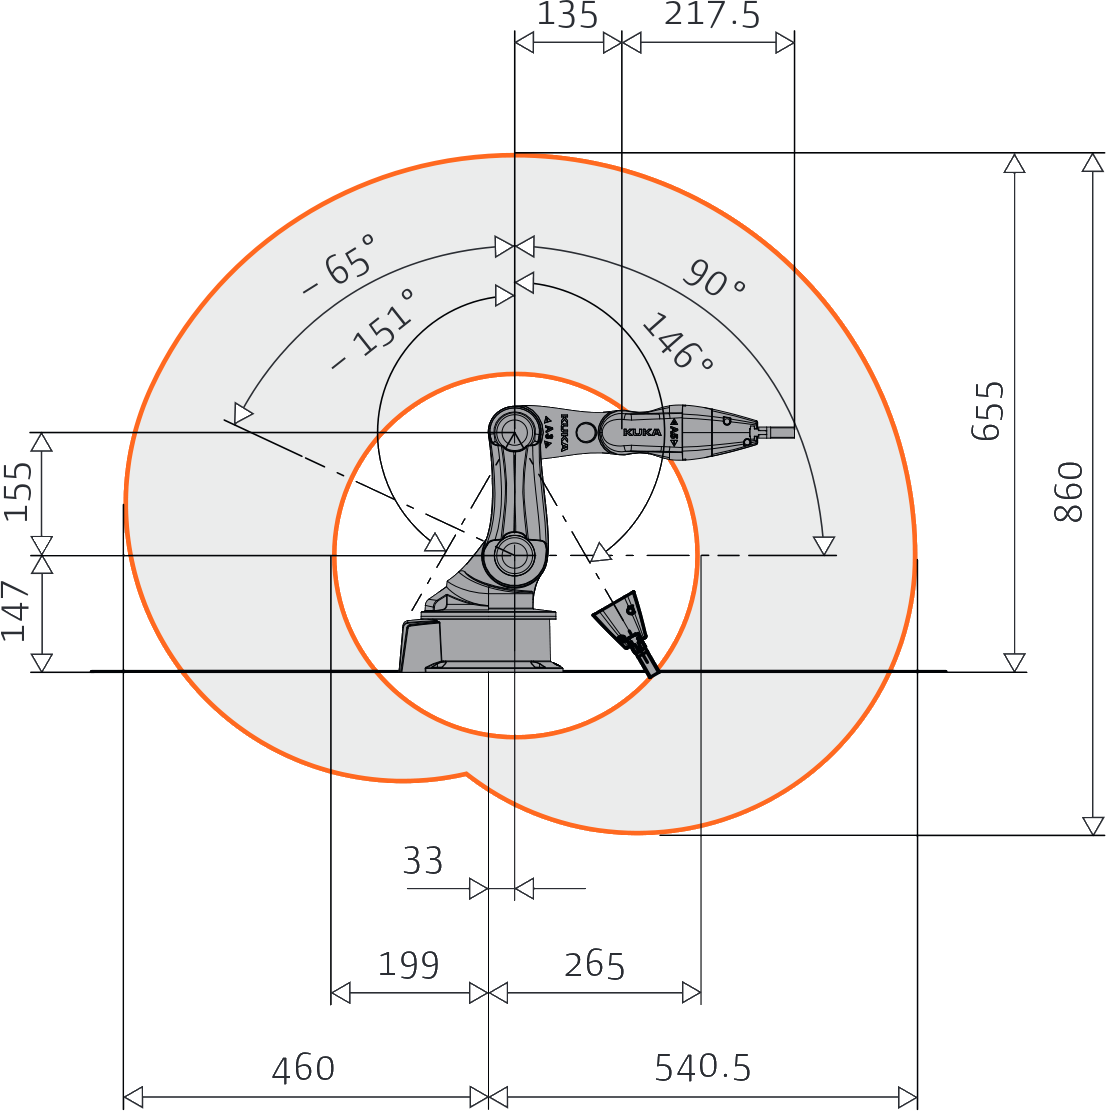
\includegraphics[scale=0.2]{Bilder/AxesYB}
\caption{Zeichnung eines Youbot-Arms und seiner fünf Rotationsachsen \cite{You}}
\label{fig:Youbot2}
\end{minipage}$
\end{figure}
%\subsection{Scitos G5}
%\begin{figure}[H] 
%\centering
%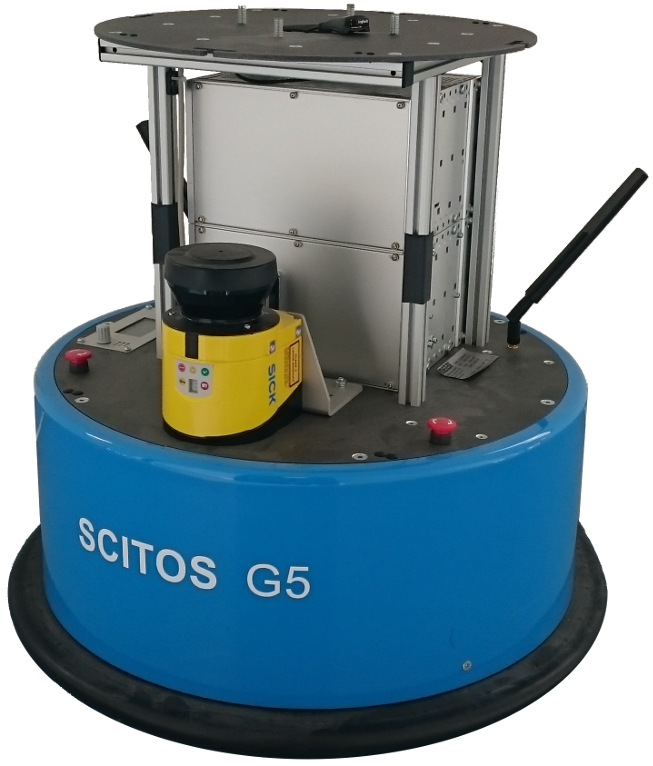
\includegraphics[scale=0.2]{Bilder/Scitos}
%\caption{Scitos G5 von der MetraLabs GmbH}
%\end{figure}
%
%\section{Verwendete Software}
%Um die Hardware zu nutzen und das geplante Konzept umzusetzen, benötigt es einer Kommunikation zwischen den Geräten und weiterer Werkzeuge zur Aufnahme von Messungen und deren Verarbeitung. Bei der Umsetzung wurde besonders auf Konfirmität der verschiedenen Systeme und deren reibungslosen Zusammenspiels geachtet. Um eine gemeinsame Basis zu schaffen, wurde das Software-Framework "`Robots Operating System"'(ROS) verwendet. Mit einem gemeinsamen Standard lassen sich die Messungen besser vergleichen, wodurch ihre Qualität und Aussagekraft zunimmt. Die Messungen müssen dabei auf der Smartphone-Plattform und den Roboter-Plattformen aufgenommen und  diese synchronisiert werden. Während ROS die übergeordnete Schnittstelle darstellt, müssen auf den einzelnen Hardware-Elementen die Messungen eigenständig durchgeführt werden. Die Messung auf dem Scitos-Roboter entfällt dabei auf die Software "`Miracenter"' und funktioniert ohne weiteres. Die Software für die Messungen auf dem Smartphone ist hingegen nicht vorgefertig und muss mithilfe eines Editors für Android-Applikationen und einer speziellen Bibliothek für die Kommunikation Smartphone $\rightarrow$ Estimote Beacon entwickelt werden.
%\subsection{ROS}
%Hier wird ROS erklärt.
%\subsection{Miracenter}
%\begin{wrapfigure}{r}{7cm}
%\centering
%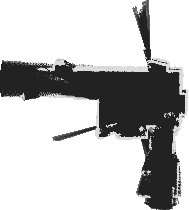
\includegraphics[scale=0.9]{Bilder/Flur}
%\caption{Grundriss eines Flures in Gebäude 29 der OvGU, Stockwerk 3}
%\label{fig:Flur}
%\end{wrapfigure}
%Mit der Software "`Miracenter"' der Firma MetraLabs GmbH ist es möglich, mit einem Scitos G5 Roboter den Grundriss eines Raumes zu erstellen. Als Sensorinformationen bezieht die Software Daten von den Inertailsensoren, Schrittmotoren und des Laserscanners und kombiniert diese zu einer Karte. Dabei wird mithilfe der Schrittmotoren der zurückgelegte Weg gemessen und diese Information mit den Inertialsensoren verbessert. Der Laserscanner sucht Erklärung der Funktionsweise des Frameworksdabei nach festen Objekten und misst die Entfernung vom Roboter zu den Objekten. Im nebenstehendem Bild ist eine solche Karte als Beispiel aufgeführt. Die Daten die Miracenter dem Nutzer zur Verfügung stellt, bestehen aus der Position des Roboters und seiner Ausrichtung in der Karte. Die Karte liegt dabei als PNG-Datei vor, wobei ein Pixel einer konstanten metrischen Länge entspricht. Die Farbwerte der Bildpunkte beschreiben zudem, ob an einer Stelle ein Hinderniss oder ein frei befahrbarer Raum vorliegt. In Abbildung \ref{fig:Flur} ist zu erkennen, dass die erstellte Karte teilweise verrauscht ist, Wände nicht gerade verlaufen, oder offene Türen und herumlaufende Personen die Messungen verfälschen. Die Karte kann dafür nach der Erstellung von jedem beliebigen Bildbearbeitungsprogramm geöffnet und verändert werden. Dabei ist darauf zu achten die Auflösung nicht zu verändern, da ansonsten die Dimensionen nicht mehr übereinstimmen. Nach der Bearbeitung der Bilddatei kann sie anschließend im Miracenter geladen werden. Mittels Mausklick in die Karte wird die ungefähre Position des Roboters bestimmt. Danach orientiert sich der Scitos automatisch und lokalisiert sich im weiteren Verlauf selbst anhand seiner Sensordaten. Nun können ihm Positionen und Ausrichtung vorgegeben werden und durch seiner internen Pfadplanung steuert er sie autonom an. Durch ein Miracenter-ROS-Interface kann dabei die interne Lokalisierung und die Vorgabe von Position und Ausrichtung vom Scitos extern übermittelt werden. Die gesamte Software ist jedoch proprietär, d.h. nicht quelloffen, sodass ein tieferer Blick in die Funktionsweise der Software dem Nutzer verwehrt bleibt.
%\subsection{Android-Studio}
%Programm zur Erstellung von Apps.
%\subsection{Estimote SDK for Android}
%Bibliothek für die Einbindung in eine Android-App. Heir kann schon auf Teile in der App eingegangen werden.
%\section{App-Entwicklung}
%Was muss die App leisten?
%\subsection{ROS-Anbindung}
%Kurze Beschreibung des Talkers.
%\subsection{Lagemessung}
%Auslesen des Gyros und der Komplementärfilterung.
%\subsection{Beacon-Detektierung}
%Probleme ansprechen mit gleichzeitiger Nutzung von WLAN undBluetooth. Am Ende ein schöner Programmablaufplan.
%
%\section{Experimente}
%\subsection{Versuchsplanung}
%Nötig?
%
%\subsection{Messung der BLE-Signalausbreitung}
%Zuerst werden zwei bis drei Distanzen und dazu die berechnete Distanz aus der App gegenübergestellt. Das wird schlecht sein und aus dem weitren Grund, dass es eine "`Black Box"' ist (d.h. man kann nicht einsehen, wie die Distanz aus dem RSSI-Wert berechnet wird), wird hier geplant ein eigenes Modell aufzustellen. Da wurde entschieden für verschiedene Distanzen nur die RSSI-Werte aufzunehmen, um später ein eigenes Modell zu implementieren.
%\begin{figure}[H] 
%\centering
%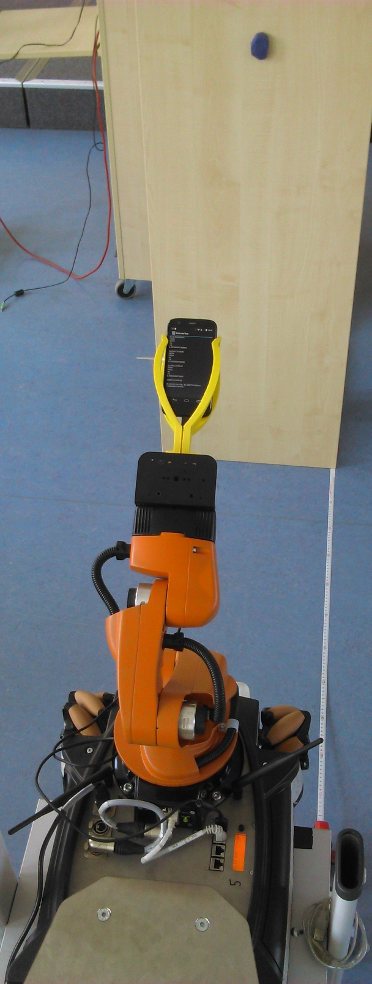
\includegraphics[scale=0.3]{Bilder/MessungDistanz1}
%\caption{Distanz-Signalstärke-Messung Bild 1}
%\end{figure}
%\begin{figure}[H] 
%\centering
%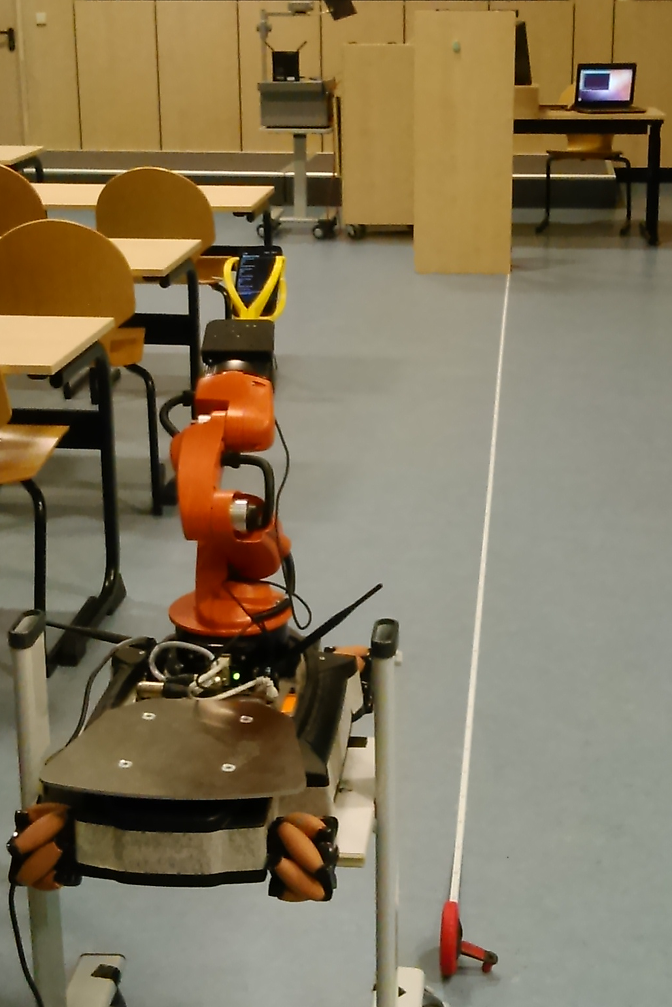
\includegraphics[scale=0.3]{Bilder/MessungDistanz2}
%\caption{Distanz-Signalstärke-Messung Bild 2}
%\end{figure}
%\begin{figure}[H] 
%\centering
%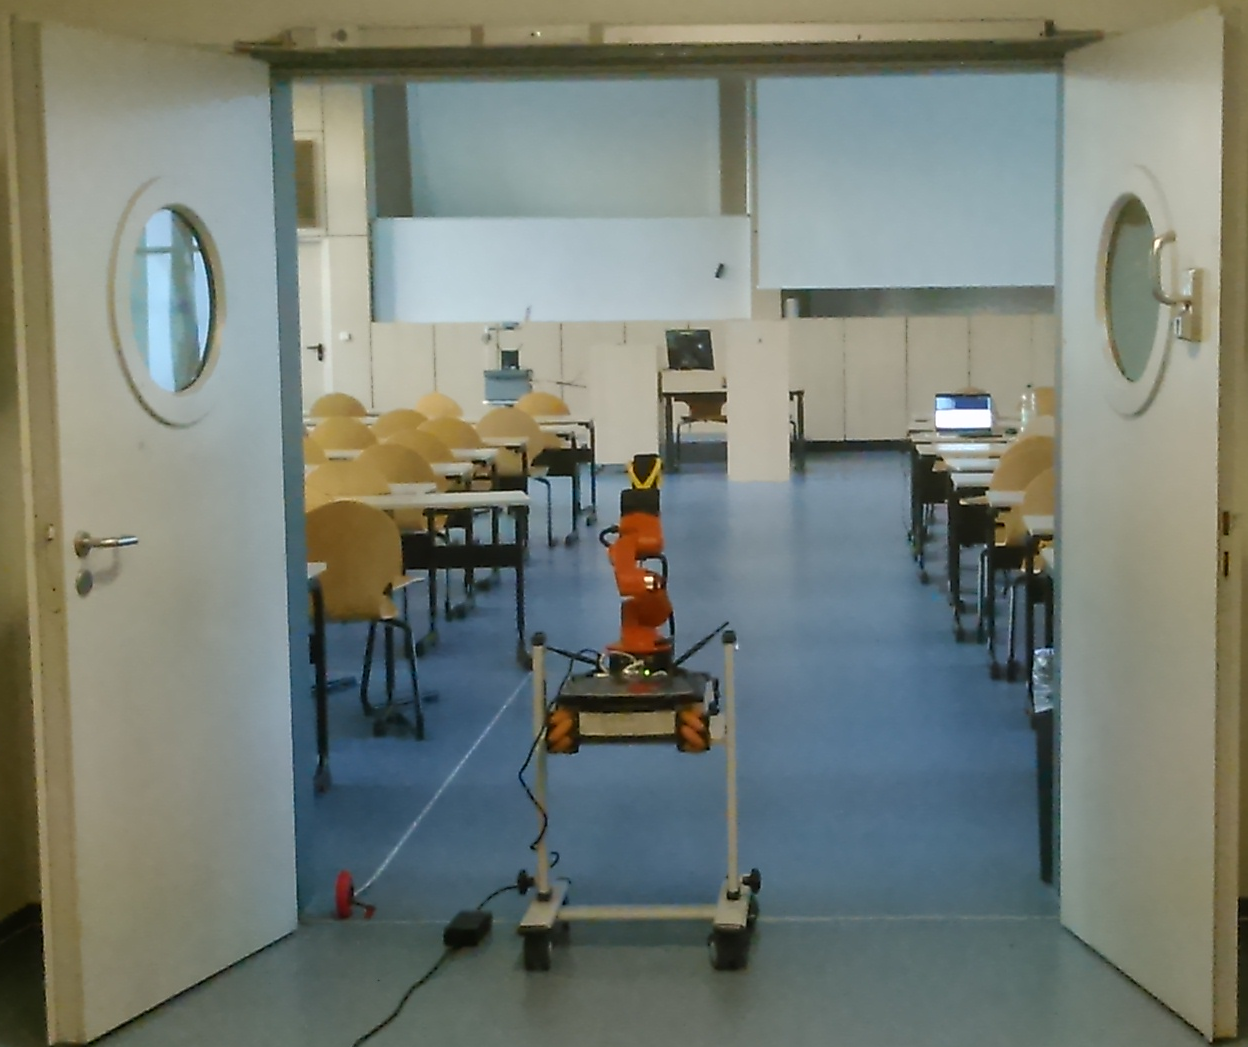
\includegraphics[scale=0.3]{Bilder/MessungDistanz3}
%\caption{Distanz-Signalstärke-Messung Bild 3}
%\end{figure}
%\subsubsection{Einfluss der Intervalllänge} 
%Wird das Rauschen vermindern.
%\subsubsection{Einfluss der Signalstärke} 
%Dies soll auch in Abhängigkeit zur Signalsstärke passieren, um dessen Ausbreitung zu erforschen.
%\subsection{Auswirkung der Smartphone-Ausrichtung}
%Hier kommen mal alle Messungen rein. Auch die mit den Beacons an allen drei Himmelsrichtungen.
%\begin{figure}[H] 
%\centering
%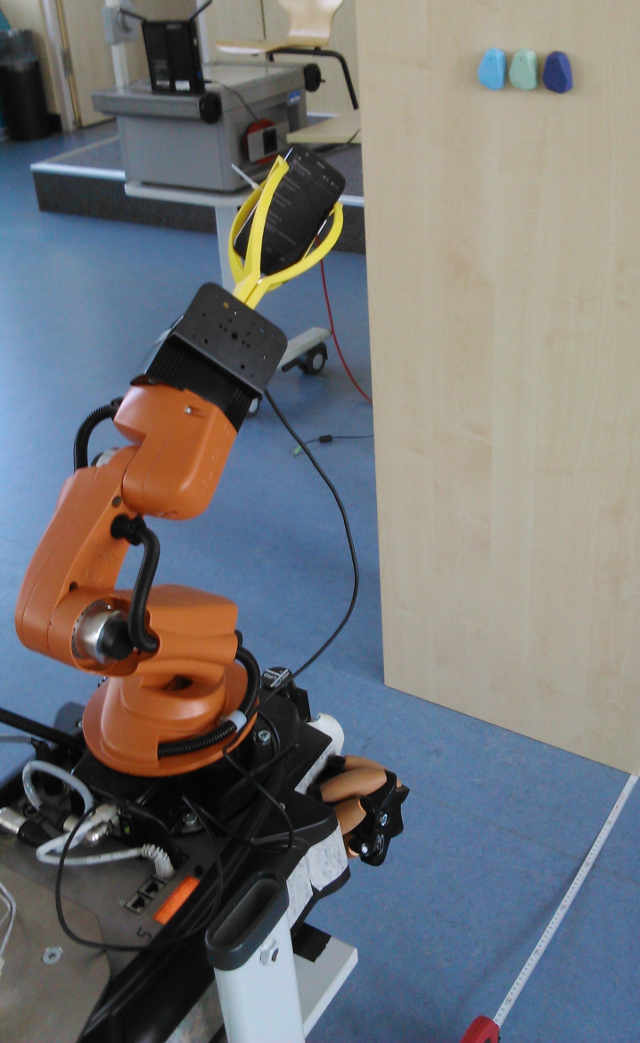
\includegraphics[scale=0.3]{Bilder/MessungDrehung}
%\caption{Distanz-Signalstärke-Messung bei unterschiedlichen Smartphone-Ausrichtungen}
%\end{figure}
%\subsection{Einfluss anderer Signalquellen} 
%Für die Erklärung aus dem zweiten Kapitel (2,4 Ghz) benötige ich auch die Störung und Interferenzen gleicher Signale. Ich muss ja schließlich erklären, warum ich nicht viele viele iBeacons nebeneinander klatschen kann, um eine möglichst genaue Standortbestimmung zu erhalten (denn die Signale stören sich untereinander). 
%ir ist z.B. aufgefallen, dass die Beacons sich gegenseitig in der Sendestärke beeinflussen. Deswegen musste ich Einzelmessungen vornehmen und hier ließe sich auch begründen nicht zu viele Beacons in der realen Anwendung zu plazieren, um durch Elektrosmog nicht zu viele Einflussfaktoren in die Lokalisierung miteinfließen zu lassen. Viel hilft hier nicht immer viel, weniger ist manchmal besser, etc.
%\begin{figure}[H] 
%\centering
%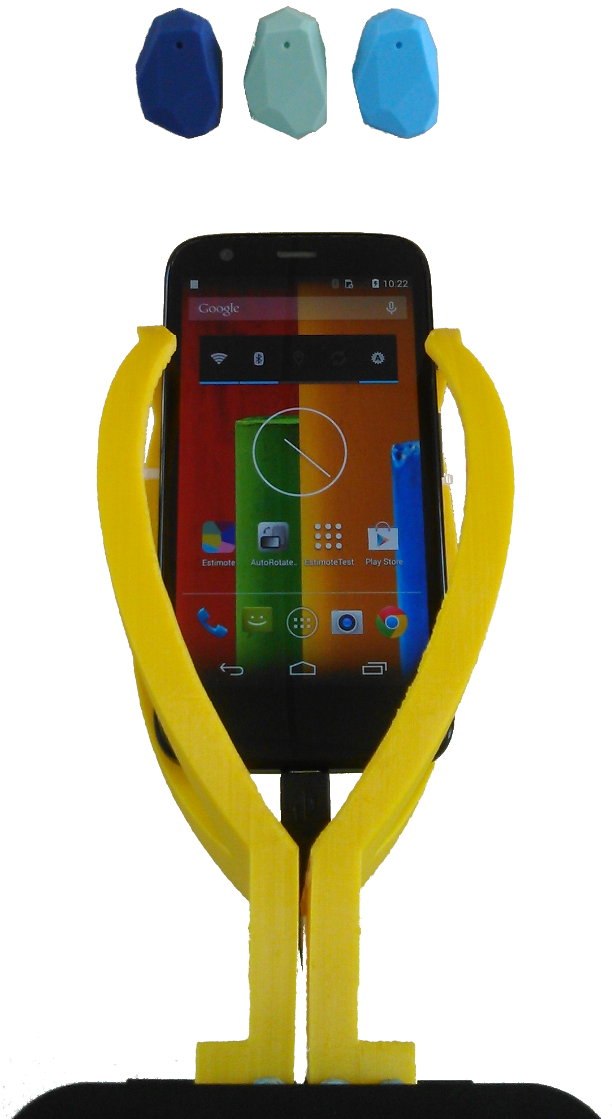
\includegraphics[scale=0.3]{Bilder/MessungBeacon3}
%\caption{Gleichzeitige Messung dreier naheliegender Beacon-Signale}
%\end{figure}
%
%\subsection{Energieverbrauch eines Beacon} 
%Der Wartungsaufwand für ein Beacon hängt maßgeblich an der Laufzeit der in jedem Beacon eingebauten Batterie ab. Die in Kapitel 1 und 2 erwähnten Einstellmöglichkeiten von Sendeleistung und der Häufigkeit von Sendeintervallen beeinflussen dabei den Stromverbrauch der Beacon und somit auch die Betriebsdauer der Batterien. Dieser Abschnitt soll sich damit beschäftigen, inwieweit sich die Parameter auf die Wartungszyklen auswirken. Dies soll später dabei helfen, zwischen der Auslegung der beiden Parameter und des gewünschten Wartungsaufwandes abwägen zu können. Denn in großen Projekten mit mehreren hundert Beacons steigt der Wartungsaufwand proportional und wenn einzelne Beacons andere Einstellungen als die Mehrheit aufweisen (um beispielsweise wichtige Gebiete besser abzudecken), wird auch der Überblick über die nötigen Wartungszyklen verloren gehen. Um die Abhängigkeiten zu veranschaulichen, wird anhand vom Datenblatt des verwendeten Hardware-Chip nRF51822\cite{nRF5} in den genutzten Beacons eine Simulation entworfen, die die Einstellmöglichkeiten als Variablen betrachtet. Als Ausgangsbasis für den Energiespeicher wird eine CR2450-Batterie mit 1,8 Wh\cite{CR2450} angenommen. Hierbei wurde nicht vom Idealzustand ausgegeangen, sondern ein üblicher Faktor von 0,7 hinzu multipliziert, um der Alterung der Zelle und weiterer Effekte Rechnung zu tragen. Durch die gering fliesenden Ströme und der minimalen Bauweise der Beacons, können auch keine direkten Messungen vorgenommen werden. Zudem kann auch nicht verifiziert werden, wie lange ein Sendeauftrag oder ein Zustand vom Prozessor dauert. Um trotzdem ein gutes Simulationsergebnis zu erreichen, muss tiefer in die Funktionsweise der Beacons geschaut werden. Als größte Unbekannte triit dabei die Sendedauer auf. Bei einer angenommenen Datenrate von 250Kbit/s  und bei einer Größe eines Datenpaketes von 38 Bytes \cite{iBPa} (siehe \ref{fig:iBPa}), dauert eine Sendesequenz rund 1 ms. Die benötigte elektrische Leistung für eine vorher definierte Sendeleistung beträgt dabei ein Vielfaches dessen und ist davon stark nichtlinear abhängig. Die dazu nötigen Beziehungen können anhand des Datenblattes des nRF51822 Chips hergeleitet werden. In diesem Fall wurde ein Polynom 4. Grades als Funktion der einstellbaren Sendeleistung aufgstellt, welches annähernd diese Abhängigkeiten beschreibt. Da die Kommunikation bidirektional ist, existiert auch ein Empfangsmodus der ebenfalls mit 1 ms Empfangsdauer angenommen wird, aber dessen Modus hingegen einen konstanten Stromverbrauch aufweist.
%\begin{figure}[H]
%\centering
%\begin{tikzpicture}
%    \node [block, fill=magenta!20, text width=2cm, minimum height=1.5cm] (Header) {\small Header \\(2 Bytes)};
%    \node [block, fill=magenta!20, right=0cm of Header, text width=3cm, minimum height=1.5cm] (MAC) {\small MAC Addresse \\(6 Bytes)};
%    \node [block, fill=magenta!20, right=0cm of MAC, text width=2cm, minimum height=1.5cm] (Data) {\small Data \\(30 Bytes)};
%    \node [block, fill=blue!20, below=1cm of Data, text width=2cm, minimum height=1.5cm] (Major) {\small Major\\ (2 Bytes)};
%    \node [block, fill=blue!20, left=0cm of Major, text width=3cm, minimum height=1.5cm] (UUID) {\small Proximity UUID \\(16 Bytes)};
%    \node [block, fill=blue!20, left=0cm of UUID, text width=3cm, minimum height=1.5cm] (Prefix) {\small iBeacon Prefix \\(9 Bytes)};
%    \node [block, fill=blue!20, right=0cm of Major, text width=2cm, minimum height=1.5cm] (Minor) {\small Minor\\ (2 Bytes)};
%    \node [block, fill=blue!20, right=0cm of Minor, text width=2cm, minimum height=1.5cm] (TX) {\small TX Power\\ (1 Bytes)};
%    \draw[very thick,->] (Data) -- (Major);
%\end{tikzpicture}
%\caption{Anteile eines Datenpaket in der Beacon-Kommunikation auf der MAC-Ebene}
%\label{fig:iBPa}
%\end{figure}
%Bei den tatsächlichen Laufzeiten des Sende- und Empfangsmodus muss jedoch ein Unsicherheitsfaktor mit eingerechnet werden, sodass nicht der berechnete Wert für eine Übertragung genommen wurde, sondern das Zweifache dessen, um ein weniger idealisiertes Bild für die einzelnen Vorgänge zu gestalten. 
%\begin{align*}
%t_{TX} &= \text{2 ms} \cdot \text{Intervalle [Hz]} \\
%t_{RX} &= \text{2 ms} \cdot \text{1 Hz} \\
%t_{CPU} &= t_{TX} + t_{RX} \\
%t_{IDLE} &= 1-t_{CPU}
%\end{align*}
%Da für den Sendevorgang noch zusätzlich der Cortex M0 Prozessor aufgeweckt werden muss und dieser das Paket vorbereitet und bis zum Ende der Sendung abwartet, muss hierfür zusätzlich der Energieverbrauch berechnet werden. Da wie erwähnt eine direkte Leistungsmessung an den Beacons durch die gering fließenden Ströme nicht möglich ist, werden aus dem Datenblatt des Prozessors diese rechnerisch ermittelt. Die aktive Phase des Prozessors für alle Operationen vor und nach einer Sendung werden dabei mit 2 ms Sekunden angenommen, welche exakt der Sende- und Empfangsdauer entspricht. Der Energiebedarf der Recheneinheit wurde im Datenblatt mit 4,1 mA bei einem Takt von 16 MHZ angegeben. So ergibt sich für den Prozessor eine Leistung von 12,3 mW. Zusätzlich wird der Stromverbrauch im IDLE-Modus (Schlafphase des Prozessors) mit 2,6 $\mu$A angegeben. Aus den genannten Gegebenheiten lassen sich nachfolgende Gleichungen erstellen und damit eine Simulation eines Lebenszyklus von einer Batterie näherungsweise bestimmen:
%\begin{align*}
%E_{Bat} &=& \text{1,8 Wh} \cdot \text{0,7} &=& \text{1,26 Wh}\\
%L_{CPU} &=& \text{4,1 mA} \cdot \text{3V} &=& \text{12,3 mW}\\
%L_{TX} &=& \text{Polynom 4. Grades (von 4,7 mA }\sim\text{ 11,8 mA)} \cdot \text{3V} &=& \text{14,1 mW} \sim \text{35,4 mW}\\
%L_{RX} &=& \text{6,1 mA} \cdot \text{3V} &=& \text{18,3 mW}\\
%L_{IDLE} &=& \text{2,6 } \mu\text{A} \cdot \text{3V} &=& \text{7,8 } \mu\text{W}
%\end{align*}
%ergeben den Zusammenhang
%\begin{align*}
%t_{Laufzeit} = \frac{E_{Bat}}{L_{CPU}\cdot t_{CPU} + L_{TX}\cdot t_{TX} + L_{RX}\cdot t_{RX} + L_{IDLE}\cdot t_{IDLE}} 
%\end{align*}
%und dies ergibt folgendes Simulationsergebniss:
%%\pgfplotsset{
%%    colormap/jet,
%%}
%%\begin{figure}[H]
%%\centering
%%\begin{tikzpicture}
%%\customrevertcolormap{jet}
%%\begin{axis}[
%%    colorbar,
%%    colorbar style={ylabel=Betriebsstunden},    
%%    view={0}{90},
%%    xlabel = {$\text{Intervalllänge [ms]}$},
%%    ylabel = {$\text{Sendeleistung [dBm]}$},
%%    %ytick pos=right,
%%    %x dir=reverse,
%%    scale=1.5   
%%]
%%\addplot3[surf, samples=40, samples y=10, domain=50:2000, domain y=-30:-20]
%%{1.8/((4.1e-3 * 3 * 4e-3  * 1000/x) + ((4.2e-5 * (-20) ^ 4 + 2.7e-3 * (-20) ^ 3 + 6.1e-2 * (-20) ^ 2 + 0.65 * (-20) + 8) * 1e-3 * 3 * 2e-3 * 1000/x) + ((6.1e-3 * 2e-3 * 2 + 2.6e-6 * (1 - (4e-3  * 1000/x + 2e-3 * 2))) * 3))};
%%\addplot3[surf, samples=40, samples y=24, domain=50:2000, domain y=-20:4]
%%{1.8/((4.1e-3 * 3 * 4e-3  * 1000/x) + ((4.2e-5 * y ^ 4 + 2.7e-3 * y ^ 3 + 6.1e-2 * y ^ 2 + 0.65 * y + 8) * 1e-3 * 3 * 2e-3 * 1000/x) + ((6.1e-3 * 2e-3 * 2 + 2.6e-6 * (1 - (4e-3  * 1000/x + 2e-3 * 2))) * 3))};
%%\end{axis}
%%\end{tikzpicture}
%%\caption{Einfluss der einstellbaren Parameter auf die Lebensdauer einer CR2450-Batterie}
%%\label{fig:iBBatLe}
%%\end{figure}
%Aufgrund der getroffenen Annahmen würde eine Batterie in den niedrigsten Einstellungen für rund 2 Jahre den Betrieb eines Beacon ermöglichen. Im realen Betrieb hatte sich gezeigt, dass eine Batterie schon nach 4 bis 5 Monaten gewechselt werden musste. Während dieser Zeit wurden die Einstellungen nicht geändert und bei einer Intervalllänge von 5 Hz und Sendeleistung von -12 dBm belassen. Beides stimmt mit der Simulation ungefähr überein, was noch kein Beweis für die Gultigkeit der Annahmen bedeutet, jedoch wird der qualitative Verlauf der wechselseitigen Beziehungen von Einstellparameter und Batterielaufzeit skizziert, welcher als Orientierung zur Auslegung der Parameter benutzt werden kann.